\documentclass{article}
\usepackage{ifthen}
\usepackage{amssymb}
\usepackage{multicol}
\usepackage{graphicx}
\usepackage[absolute]{textpos}
\usepackage{amsmath, amscd, amssymb, amsthm, latexsym}
\usepackage{xspace,rotating,dsfont,ifthen}
\usepackage[spanish,activeacute]{babel}
\usepackage[utf8]{inputenc}
\usepackage{pgfpages}
\usepackage{pgf,pgfarrows,pgfnodes,pgfautomata,pgfheaps,xspace,dsfont}
\usepackage{listings}
\usepackage{multicol}
\usepackage{todonotes}
\usepackage{url}
\usepackage{float}
\usepackage{framed,mdframed}
\usepackage{cancel}

\usepackage[strict]{changepage}


\makeatletter


\newcommand\hfrac[2]{\genfrac{}{}{0pt}{}{#1}{#2}} %\hfrac{}{} es un \frac sin la linea del medio

\newcommand\Wider[2][3em]{% \Wider[3em]{} reduce los m\'argenes
\makebox[\linewidth][c]{%
  \begin{minipage}{\dimexpr\textwidth+#1\relax}
  \raggedright#2
  \end{minipage}%
  }%
}


\@ifclassloaded{beamer}{%
  \newcommand{\tocarEspacios}{%
    \addtolength{\leftskip}{4em}%
    \addtolength{\parindent}{-3em}%
  }%
}
{%
  \usepackage[top=1cm,bottom=2cm,left=1cm,right=1cm]{geometry}%
  \usepackage{color}%
  \newcommand{\tocarEspacios}{%
    \addtolength{\leftskip}{3em}%
    \setlength{\parindent}{0em}%
  }%
}

\usepackage{caratula}
\usepackage{enumerate}
\usepackage{hyperref}
\usepackage{graphicx}
\usepackage{amsfonts}
\usepackage{enumitem}
\usepackage{amsmath}

\decimalpoint
\hypersetup{colorlinks=true, linkcolor=black, urlcolor=blue}
\setlength{\parindent}{0em}
\setlength{\parskip}{0.5em}
\setcounter{tocdepth}{2} % profundidad de indice
\setcounter{section}{5} % nro de section
\renewcommand{\thesubsubsection}{\thesubsection.\Alph{subsubsection}}
\graphicspath{ {images/} }

% End latex config

\begin{document}

\titulo{Práctica 6}
\fecha{2do cuatrimestre 2021}
\materia{Álgebra I}
\integrante{Yago Pajariño}{546/21}{ypajarino@dc.uba.ar}

%Carátula
\maketitle
\newpage

%Indice
\tableofcontents
\newpage

% Aca empieza lo propio del documento
\section{Práctica 6}

\subsection{Ejercicio 1}

\subsubsection{Pregunta i}

Paso a polares:
\begin{itemize}
    \item $ 5i = 5(\cos(\frac{\pi}{2}) + i\sin(\frac{\pi}{2})) $
    \item $ (1+i)^4 = (\sqrt{2})^4 .(\cos(\pi)+i\sin(\pi)) $
\end{itemize}

Luego,
\begin{align*}
    z &= 4.5(\cos(\pi + \frac{\pi}{2})+i\sin(\pi +\frac{\pi}{2})) \\
    &= 20(\cos(\frac{3\pi}{2})+i\sin(\frac{3\pi}{2})) \\
\end{align*}

Así,
\begin{itemize}
    \item $ Re(z) = 20. \cos(\frac{3\pi}{2}) = 0 $
    \item $ Im(z) = 20. \sin(\frac{3\pi}{2}) = -20 $
    \item $ |z| = 20 $
    \item $ Re(z^{-1}) = 0 $
    \item $ iz = 20(\cos(2\pi)+i\sin(2\pi)) \implies Im(iz) = 0 $
\end{itemize}

\subsubsection{Pregunta ii}

\begin{align*}
    z &= (\sqrt[]{2} + \sqrt[]{3}i)^2.(\overline{1-3i}) \\
    &= (2 + 2\cdot \sqrt[]{2} \cdot\sqrt[]{3}i - 3).(1 + 3i) \\
    &= (-1 + 2\cdot \sqrt[]{6}i).(1 + 3i) \\
    &= -1 - 3i + 2 \cdot\sqrt[]{6}i - 6 \cdot \sqrt[]{6} \\
    &= -1 - 6 \cdot \sqrt[]{6} + (2 \cdot\sqrt[]{6} - 3)i \\
\end{align*}

\begin{itemize}
    \item $ Re(z) = -1 - 6 \cdot \sqrt[]{6} $
    \item $ Im(z) = 2 \cdot\sqrt[]{6} - 3 $
    \item $ |z| = \sqrt{(-1 - 6 \cdot \sqrt[]{6})^2 + (2 \cdot\sqrt[]{6} - 3)^2} = \sqrt[]{250} = 5\cdot\sqrt[]{10} $
\end{itemize}

\subsubsection{Pregunta iii}

Paso a polares,

$ i^{17} = \cos(17.\frac{\pi}{2}) + i\sin(17\frac{\pi}{2}) $

$ \frac{1}{2} = \frac{1}{2}.(\cos(0) + i\sin(0)) $

$ i = \cos(\frac{\pi}{2}) +i\sin(\frac{\pi}{2}) $

$ (1-i)^3 = (\sqrt[]{2})^3(\cos(3.\frac{7}{4}\pi)+i\sin(3.\frac{7}{4}\pi)) $

Luego,
\begin{align*}
    \frac{1}{2} . i . (1+i)^3 &= \frac{1}{2}.(\sqrt[]{2})^3.\left(\cos(\frac{\pi}{2} + \frac{21}{4}\pi) +i\sin(\frac{\pi}{2} + \frac{21}{4}\pi)\right) \\
    &= \frac{\sqrt[]{2}^3}{2}.\left(\cos\left(\frac{23}{4}\pi\right) +i\sin\left(\frac{23}{4}\pi\right)\right) \\
\end{align*}
Entonces,
\begin{align*}
    z &= \frac{\sqrt[]{2}^3}{2}.\left(\cos\left((\frac{17}{2} + \frac{23}{4})\pi\right) +i\sin\left((\frac{17}{2} + \frac{23}{4})\pi\right)\right) \\
    &= \frac{\sqrt[]{2}^3}{2}.\left(\cos\left(\frac{57}{4}\pi\right) +i\sin\left(\frac{57}{4}\pi\right)\right) \\
\end{align*}

\begin{itemize}
    \item $ Re(z) = \frac{\sqrt[]{2}^3}{2} . \cos\left(\frac{57}{4}\pi\right) $
    \item $ Im(z) = \frac{\sqrt[]{2}^3}{2} . \sin\left(\frac{57}{4}\pi\right) $
    \item $ |z| = \frac{\sqrt[]{2}^3}{2} $
    \item $ Re(z^{-1}) = \cos\left(\frac{57}{4}\pi\right) $
    \item $ Im(iz) = \frac{\sqrt[]{2}^3}{2} . \sin\left(\frac{59}{4}\pi\right) $
\end{itemize}

\subsubsection{Pregunta iv}
TODO

\subsubsection{Pregunta v}
TODO

\subsection{Ejercicio 2}

\begin{enumerate}
    \item 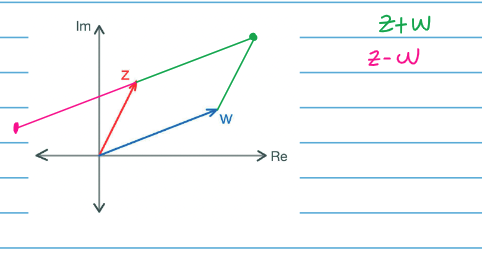
\includegraphics[width=250px]{6.2.1}
    \item 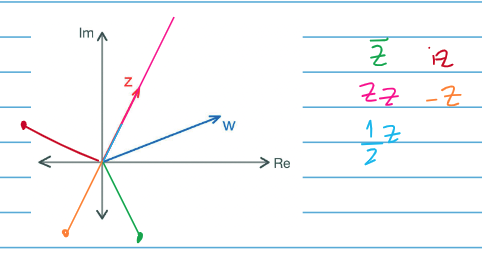
\includegraphics[width=250px]{6.2.2}
    \item 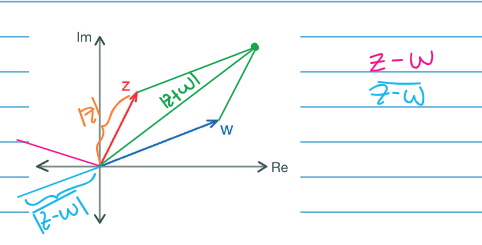
\includegraphics[width=250px]{6.2.3}
\end{enumerate}

\subsection{Ejercicio 3}

\subsubsection{Pregunta i}

$ z^2 = -36 $

Se que $ z = a+bi $ con $ (a,b) \in \mathbb{R}^2 $

Luego busco los $z$ tales que $z^2 = -36 $

\begin{align*}
    z^2 = -36 \iff z^2 &= (a+bi)^2 \\
    &= a^2 - b^2 + 2abi \\
\end{align*}

También se que el módulo debe ser igual $ |z^2| = |-36| $,

$ |z^2| = |z|^2 = (\sqrt{a^2+b^2})^2 = a^2+b^2 $ \\
$ |-36| = 36 $

Usando la igualdad de números complejos,

$ \begin{cases}
    a^2-b^2 = -36 \\
    2ab = 0 \\
    a^2+b^2 = 36 \\
\end{cases} $

Sumando (1) y (3) $ 2a^2 = 0 \iff a = 0 $

Restando (1) a (3) $ 2b^2 = 2.36 \iff b = \pm 36 $

Luego $ z = a+bi $ con los valores de a y b hallados resulta en

Rta.: $ z_1 = 6i; z_2 = -6i $

\subsubsection{Pregunta ii}

$ z^2 = i $

Se que $ z = a+bi $ con $ (a,b) \in \mathbb{R}^2 $

También se que el módulo debe ser igual $ |z^2| = |i| $,

$ |z^2| = |z|^2 = (\sqrt{a^2+b^2})^2 = a^2+b^2 $ \\
$ |i| = 1 $

Usando la igualdad de números complejos,

$ \begin{cases}
    a^2-b^2 = 0 \\
    2ab = 1 \\
    a^2+b^2 = 1 \\
\end{cases} $

Sumando (1) y (3) $ 2a^2 = 1 \iff a = \pm \frac{1}{\sqrt[]{2}} $

Restando (1) a (3) $ 2b^2 = 1 \iff b = \pm \frac{1}{\sqrt[]{2}} $

Usando (2) se que $ 2ab > 0 \iff (a > 0 \wedge b > 0) \vee (a < 0 \wedge b < 0) $

Rta.: $ z_1 = \frac{1}{\sqrt[]{2}} + \frac{1}{\sqrt[]{2}}i; z_2 = -\frac{1}{\sqrt[]{2}} - \frac{1}{\sqrt[]{2}}i $

\subsubsection{Pregunta iii}

$ z^2 = 7+24i $

Se que $ z = a+bi $ con $ (a,b) \in \mathbb{R}^2 $

También se que el módulo debe ser igual $ |z^2| = |7+24i| $,

$ |z^2| = |z|^2 = (\sqrt{a^2+b^2})^2 = a^2+b^2 $

$ |7+24i| = \sqrt[]{7^2+24^2} = \sqrt[]{49+576} = 25 $

Usando la igualdad de números complejos,

$ \begin{cases}
    a^2-b^2 = 7 \\
    2ab = 24 \\
    a^2+b^2 = 25 \\
\end{cases} $

Sumando (1) y (3) $ 2a^2 = 32 \iff a = \pm 4 $

Restando (1) a (3) $ 2b^2 = 18 \iff b = \pm 3 $

Usando (2) se que $ 2ab > 0 \iff (a > 0 \wedge b > 0) \vee (a < 0 \wedge b < 0) $

Rta.: $ z_1 = 4+3i; z_2 = -4-3i $

\subsubsection{Pregunta iv}

$ z^2 + 15 - 8i = 0 \iff z^2 = -15+8i $

Se que $ z = a+bi $ con $ (a,b) \in \mathbb{R}^2 $

También se que el módulo debe ser igual $ |z^2| = |-15+8i| $,

$ |z^2| = |z|^2 = (\sqrt{a^2+b^2})^2 = a^2+b^2 $

$ |-15+8i| = \sqrt[]{(-15)^2+8^2} = \sqrt[]{225 + 64} = 17 $

Usando la igualdad de números complejos,

$ \begin{cases}
    a^2-b^2 = -15 \\
    2ab = 8 \\
    a^2+b^2 = 17 \\
\end{cases} $

Sumando (1) y (3) $ 2a^2 = 2 \iff a = \pm 1 $

Restando (1) a (3) $ 2b^2 = 16 \iff b = \pm 4 $

Usando (2) se que $ 2ab > 0 \iff (a > 0 \wedge b > 0) \vee (a < 0 \wedge b < 0) $

Rta.: $ z_1 = 1+4i; z_2 = -1-4i $

\subsection{Ejercicio 4}

\subsubsection{Pregunta i}

$ z = (2+2i)(\sqrt[]{3}-i) $

Busco la forma polar de cada factor.
\begin{align*}
    2+2i &= \sqrt[]{8}. e^{\frac{\pi}{4}i} \\
    \sqrt[]{3} - i &= 2.e^{\frac{11}{6}\pi i}
\end{align*}
Por DeMoivre,
\begin{align*}
    z &= (2+2i)(\sqrt[]{3}-i) \\
    &= \sqrt[]{8}. 2. e^{\frac{\pi}{4}i + \frac{11}{6}\pi i} \\
    &= 2 \cdot \sqrt[]{8} e^{\frac{1}{12}\pi i}
\end{align*}
Luego,
\begin{itemize}
    \item $ |z| = 4\cdot \sqrt[]{2} $
    \item $ \theta = \frac{1}{12}\pi $
\end{itemize}

\subsubsection{Pregunta ii}

$ z = (-1+\sqrt[]{3}i)^5 $
\begin{align*}
    -1+\sqrt[]{3}i &= 2\cdot e^{(\pi - \frac{1}{3}\pi)i} \\
    &= 2\cdot e^{\frac{2}{3}\pi i } 
\end{align*}
Luego,
\begin{align*}
    z &= (-1+\sqrt[]{3}i)^5 \\
    &= (2\cdot e^{\frac{2}{3}\pi i })^5 \\
    &= 2^5\cdot e^{\frac{10}{3}\pi i }
\end{align*}
Por lo tanto,
\begin{itemize}
    \item $ |z| = 2^5 $
    \item $ \theta = \frac{4}{3}\pi $
\end{itemize}

\subsubsection{Pregunta iii}

$ z = (-1+\sqrt[]{3}i)^{-5} $
\begin{align*}
    z &= (-1+\sqrt[]{3}i)^{-5} \\
    &= (2\cdot e^{\frac{2}{3}\pi i })^{-5} \\
    &= 2^{-5}\cdot e^{\frac{-10}{3}\pi i }
\end{align*}
Por lo tanto,
\begin{itemize}
    \item $ |z| = \frac{1}{2^5} $
    \item $ \theta = \frac{2}{3}\pi $
\end{itemize}

\subsubsection{Pregunta iv}

$ z = \frac{1+\sqrt[]{3}i}{1-i} $

Busco las expresiones polares.
\begin{align*}
    1+\sqrt[]{3}i &= 2. e^{\frac{\pi}{3}i} \\
    1-i &= \sqrt[]{2}. e^{\frac{7}{4}\pi i}
\end{align*}
Luego,
\begin{align*}
    z &= \frac{1+\sqrt[]{3}i}{1-i} \\
    &= \frac{2}{\sqrt[]{2}} \cdot e^{(\frac{1}{3} - \frac{7}{4})\pi i} \\
    &= \frac{2}{\sqrt[]{2}} \cdot e^{\frac{-17}{12}\pi i}
\end{align*}
Por lo tanto,
\begin{itemize}
    \item $ |z| = \frac{2}{\sqrt[]{2}} $
    \item $ \theta = \frac{7}{12}\pi $
\end{itemize}

\subsection{Ejercicio 5}

\subsubsection{Pregunta i}

$ Re(z) = x \wedge Im(z) = y \implies x+5y \leq 8 \iff y \leq -\frac{1}{5}x + \frac{8}{5}$

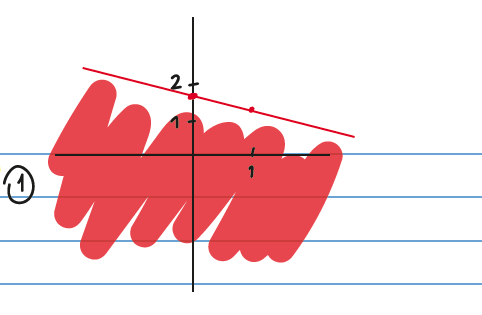
\includegraphics[width=250px]{6.5.1}

\subsubsection{Pregunta ii}

\begin{itemize}
    \item $ |z| = 2 $ define una circunferencia de radio 2.
    \item $ \frac{\pi}{4} \leq arg(z) \leq \frac{2\pi}{3} $ define un arco de angulo barrido.
\end{itemize}

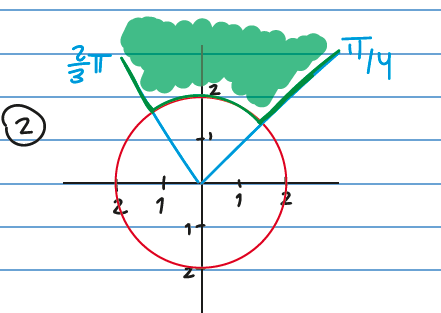
\includegraphics[width=250px]{6.5.2}

\subsubsection{Pregunta iii}
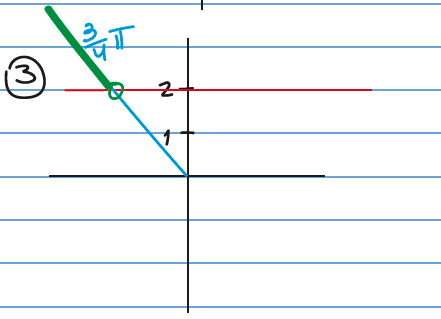
\includegraphics[width=250px]{6.5.3}

\subsubsection{Pregunta iv}
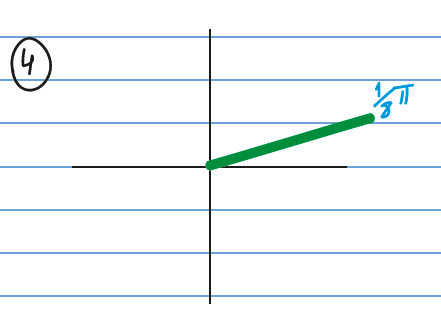
\includegraphics[width=250px]{6.5.4}

\subsection{Ejercicio 6}

\subsubsection{Pregunta i}

$ z = (\frac{1+\sqrt[]{3}i}{1-i})^{17} $

Sea $ w = \frac{1+\sqrt[]{3}i}{1-i} $

Busco las expresiones polares.
\begin{align*}
    1+\sqrt[]{3}i &= 2. e^{\frac{\pi}{3}i} \\
    1-i &= \sqrt[]{2}. e^{\frac{7}{4}\pi i}
\end{align*}
Luego,
\begin{align*}
    w &= \frac{1+\sqrt[]{3}i}{1-i} \\
    &= \frac{2}{\sqrt[]{2}} \cdot e^{(\frac{1}{3} - \frac{7}{4})\pi i} \\
    &= \frac{2}{\sqrt[]{2}} \cdot e^{\frac{7}{12}\pi i}
\end{align*}
Por lo tanto,
\begin{align*}
    z &= w^{17} \\
    &= \left(\frac{2}{\sqrt[]{2}} \cdot e^{\frac{7}{12}\pi i}\right)^{17} \\
    &= \left(\frac{2}{\sqrt[]{2}}\right)^{17} \cdot e^{\frac{17.7}{12}\pi i} \\
    &= \left(\frac{2}{\sqrt[]{2}}\right)^{17} \cdot e^{\frac{23}{12}\pi i} \\
\end{align*}
Por lo tanto,
$ z = \left(\frac{2}{\sqrt[]{2}}\right)^{17} \cdot \cos(\frac{23}{12}\pi i) + \left(\frac{2}{\sqrt[]{2}}\right)^{17} \cdot \sin(\frac{23}{12}\pi i) $

\subsubsection{Pregunta ii}

$ z = (-1+\sqrt[]{3}i)^{n} $

$ -1+\sqrt[]{3}i = 2\cdot e^{\frac{2}{3}\pi i} $

$ (-1+\sqrt[]{3}i)^{n} = 2^n \cdot e^{\frac{2n}{3}\pi i} $

Luego $ 0 \leq \frac{2n}{3}\pi i < 2\pi \iff 0 \leq n < 3 $

Por lo tanto,
\begin{itemize}
    \item $ n = 0 \implies z = 1 $
    \item $ n = 1 \implies z = 2\cdot e^{\frac{2}{3}\pi i} = -1+\sqrt[]{3}i $
    \item $ n = 1 \implies z = 4\cdot e^{\frac{4}{3}\pi i} = -2+ 2 \cdot \sqrt[]{3}i $
\end{itemize}

\end{document}
